		\begin{enumerate}
			\item
			\begin{enumerate}
				\item $(A(0),B(0)) = (0,1)$
				\item The solution is periodic because $(A(0),B(0))=(A(8),B(8))$
				\item \phantom{x}

				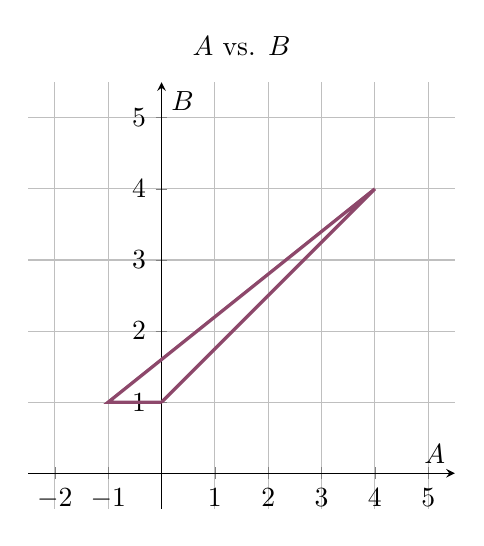
\begin{tikzpicture}
					\begin{axis}[
						title={$A$ vs. $B$},
						width=7cm,
						height=7cm,
						xmin=-2.5,xmax=5.5,
						ymin=-.5,
						ymax=5.5, xmajorgrids, ymajorgrids,
						xtick={-10,...,10}, ytick={0,1,...,10},
						axis lines=middle,
						samples=5, domain=-5:5,
						xlabel={$A$},
						ylabel={$B$}
						]
						
						%\addplot[red, thick] coordinates {(0,0) (2,4) (5,-1) (8,0)};
						%\addplot[green!50!black, thick] coordinates {(0,1) (2,4) (5,1) (8,1)};
						\addplot[magenta!50!black, very thick] coordinates {(0,1) (4,4) (-1,1) (0,1)};
					\end{axis}
				\end{tikzpicture}%
				
			\end{enumerate}
			\item \begin{enumerate}
				\item \phantom{x}

				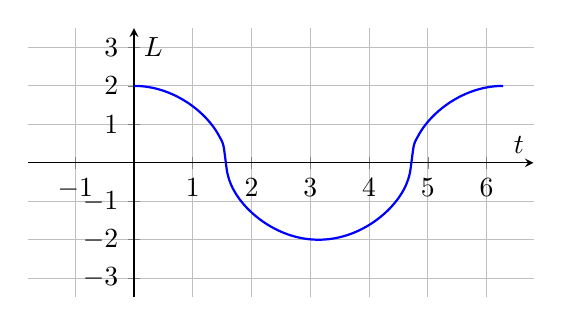
\begin{tikzpicture}
					\begin{axis}[
						width=8cm,
						height=5cm,
						xmin=-1.8,xmax=6.8,			
						ymin=-3.5,
						ymax=3.5, xmajorgrids, ymajorgrids,
						xtick={-5,...,10}, ytick={-10,...,10},
						axis lines=middle,
						samples=5, domain=-5:5,
						xlabel={$t$},
						ylabel={$L$}
						]
						
						\addplot [
							domain=0:2*pi,
							samples=100,
							smooth,
							thick,
							blue
						] 
						({x}, {2*sign(cos(deg(x)))*abs(cos(deg(x)))^(1/2)});
						%({cos(deg(x)) / (1 + sin(deg(x))^2)}, {cos(deg(x)) * sin(deg(x)) / (1 + sin(deg(x))^2)});
					\end{axis}
				\end{tikzpicture}
				~~~~
				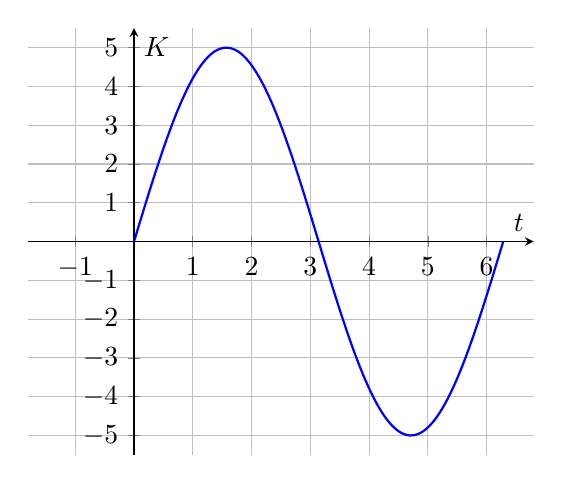
\begin{tikzpicture}
					\begin{axis}[
						width=8cm,
						height=7cm,
						xmin=-1.8,xmax=6.8,			
						ymin=-5.5,
						ymax=5.5, xmajorgrids, ymajorgrids,
						xtick={-5,...,10}, ytick={-10,...,10},
						axis lines=middle,
						samples=5, domain=-5:5,
						xlabel={$t$},
						ylabel={$K$}
						]
						
						\addplot [
							domain=0:2*pi,
							samples=100,
							smooth,
							thick,
							blue
						] 
						({x}, {5*sin(deg(x))});
						%({cos(deg(x)) / (1 + sin(deg(x))^2)}, {cos(deg(x)) * sin(deg(x)) / (1 + sin(deg(x))^2)});
					\end{axis}
				\end{tikzpicture}
				
				\item \phantom{x}

				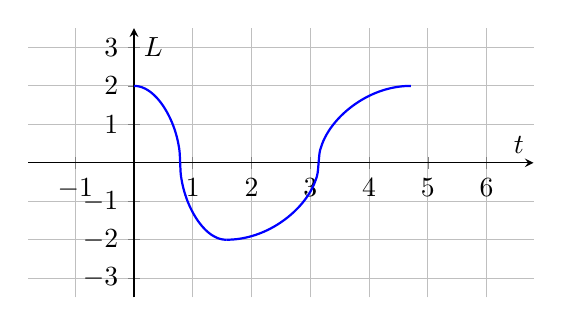
\begin{tikzpicture}
					\begin{axis}[
						width=8cm,
						height=5cm,
						xmin=-1.8,xmax=6.8,			
						ymin=-3.5,
						ymax=3.5, xmajorgrids, ymajorgrids,
						xtick={-5,...,10}, ytick={-10,...,10},
						axis lines=middle,
						samples=5, domain=-5:5,
						xlabel={$t$},
						ylabel={$L$}
						]
						
						\addplot [
							domain=0:pi/2,
							samples=100,
							smooth,
							thick,
							blue
						] 
						({x}, {2*sign(cos(deg(2*x)))*abs(cos(deg(2*x)))^(1/2)});
						\addplot [
							domain=pi:2*pi,
							samples=100,
							smooth,
							thick,
							blue
						] 
						({x-pi/2}, {2*sign(cos(deg(x)))*abs(cos(deg(x)))^(1/2)});
						%({cos(deg(x)) / (1 + sin(deg(x))^2)}, {cos(deg(x)) * sin(deg(x)) / (1 + sin(deg(x))^2)});
					\end{axis}
				\end{tikzpicture}
				~~~~
				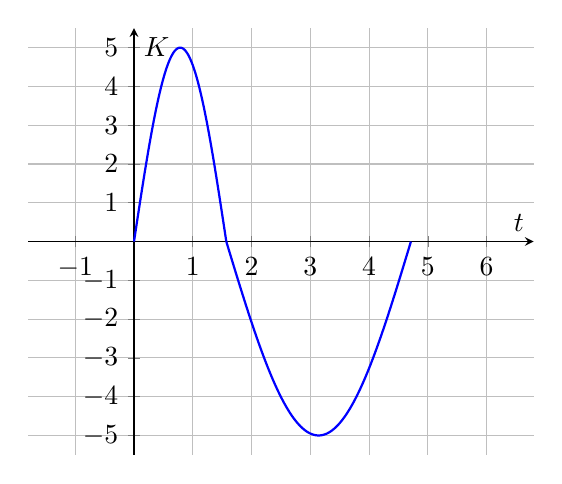
\begin{tikzpicture}
					\begin{axis}[
						width=8cm,
						height=7cm,
						xmin=-1.8,xmax=6.8,			
						ymin=-5.5,
						ymax=5.5, xmajorgrids, ymajorgrids,
						xtick={-5,...,10}, ytick={-10,...,10},
						axis lines=middle,
						samples=5, domain=-5:5,
						xlabel={$t$},
						ylabel={$K$}
						]
						
						\addplot [
							domain=0:pi/2,
							samples=100,
							smooth,
							thick,
							blue
						] 
						({x}, {5*sin(deg(2*x))});
						\addplot [
							domain=pi:2*pi,
							samples=100,
							smooth,
							thick,
							blue
						] 
						({x-pi/2}, {5*sin(deg(x))});
						%({cos(deg(x)) / (1 + sin(deg(x))^2)}, {cos(deg(x)) * sin(deg(x)) / (1 + sin(deg(x))^2)});
					\end{axis}
				\end{tikzpicture}
			\end{enumerate}

			\item \begin{enumerate}
				\item You can always create a graph in phase space from component graphs, but not the other way around.
				Graphs in phase space loose all ``speed'' information, but component graphs have information about the
				speed/velocity of a solution.

				\item Component graphs allow you to visualize the relationship among different quantities in ways
				that may not be obvious from analyzing component graphs. Component graphs, on the other hand, contain
				complete information about a solution, including its speed/velocity.
			\end{enumerate}

			\item
			\begin{enumerate}
				\item \phantom{x}

				\begin{center}
				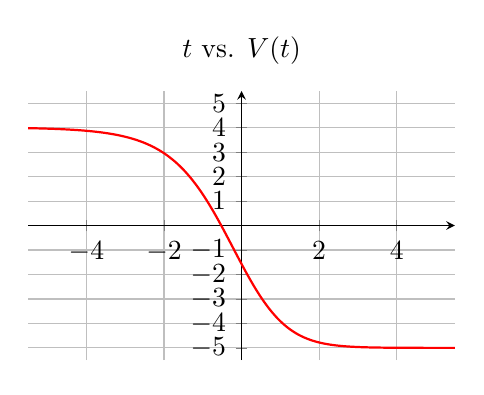
\begin{tikzpicture}
					\begin{axis}[
						title={$t$ vs. $V(t)$},
						width=7cm,
						height=5cm,
						xmin=-5.5,xmax=5.5,
						ymin=-5.5,
						ymax=5.5, xmajorgrids, ymajorgrids,
						axis lines=middle,
						ytick={-5,...,5},
						samples=200, domain=-20:20, smooth]
						
						\addplot[red, thick] {5*sin(deg((pi-0.64)/(1+exp(-x))-3*pi/2+0.64))};
					\end{axis}
				\end{tikzpicture}%
				~~~~~~~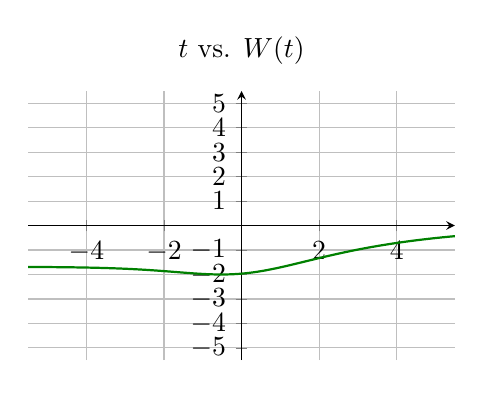
\begin{tikzpicture}
					\begin{axis}[
						title={$t$ vs. $W(t)$},
						width=7cm,
						height=5cm,
						xmin=-5.5,xmax=5.5,
						ymin=-5.5,
						ymax=5.5, xmajorgrids, ymajorgrids,
						axis lines=middle,
						ytick={-5,...,5},
						samples=200, domain=-20:20, smooth]
						
						\addplot[green!50!black, thick] {-2*(abs(cos(deg((pi-0.64)/(1+exp(-x))-3*pi/2+0.64))))^(1/3)};
					\end{axis}
				\end{tikzpicture}
				\end{center}
				\item For any one-to-one and onto function $f$, the graph of $\vec r$ and $\vec r\circ f$ will be the same,
				with a possible change in domain. We want to change the domain from $(-3\pi/2+0.64, -\pi/2)$ to $\R$, which
				means we need to find a function that is one-to-one and onto from $\R$ to $(-3\pi/2+0.64, -\pi/2)$. 
				We can do this with the function
				\[
					d(t) = \frac{\pi-0.64}{1+e^{-x}}-\frac{3\pi}{2}+0.64.
				\]
				Then $\vec q=\vec r\circ d$.
				\item We can come up with a differential equation by computing $[\vec r\circ f]'$. Doing so we see
				\[
					V'(t) = \frac{12.508\, e^t \cos\left(4.07239 - \frac{2.50159 e^t}{1 + e^t}\right)}{(1 + e^t)^2}
				\]
				%(1.66773 E^x Sin[4.07239 - (2.50159 E^x)/(1 + E^x)])/((1. + E^x)^2 Cos[4.07239 - (2.50159 E^x)/(1 + E^x)]^(2/3))
				\[
				W'(t) = 
				\frac{1.66773\, e^t \sin\left(4.07239 - \frac{2.50159 e^t}{1 + e^t}\right)}{(1 + e^t)^2 \cos\left(4.07239 - \frac{2.50159 e^t}{1 + e^t}\right)^{\frac{2}{3}}}
				\]

				\item We can come up with a different set of equations by stretching the domain, for example, by multiplying by $2$.
				We then have
				\[
					V_{\text{new}}'(t) = [V(2t)]'=2V'(2t)
				\]
				\[
					W_{\text{new}}'(t) = [W(2t)]'=2W'(2t)
				\]
			\end{enumerate}
			
			%\item \begin{enumerate}
			%	\item The equilibrium points are labelled below.

			%	
			%	\hspace{-1.5em}\begin{tikzpicture}[scale=.6, blue]
			%		% Define the vector field function
			%		% based on
			%		% https://www.desmos.com/calculator/o3xjzddojw
			%		% x' = (x+2.87)*y*(x+8.63)
			%		% y' = x*(y+7.23)*(y-4.27)
			%		\def\vectorfieldx(#1,#2){(#1 + 2.87) * (#2) * (#1 + 8.63) / 200}
			%		\def\vectorfieldy(#1,#2){(#1) * (#2 + 7.23) * (#2 - 4.27) / 200}

			%		% Draw the vector field
			%		\foreach \x in {-11,-10.4,...,10}
			%			\foreach \y in {-10,-9.4,...,10}
			%			{
			%				% Calculate the vector at (\x, \y)
			%				\pgfmathsetmacro\vx{\vectorfieldx(\x,\y)}
			%				\pgfmathsetmacro\vy{\vectorfieldy(\x,\y)}
			%				
			%				% Normalize the vector for consistent arrow lengths
			%				\pgfmathsetmacro\norm{sqrt(\vx*\vx + \vy*\vy + 0.01)}
			%				\pgfmathsetmacro\scaleChange{atan(\norm)/100/\norm}
			%				\pgfmathsetmacro\vx{\vx*\scaleChange}
			%				\pgfmathsetmacro\vy{\vy*\scaleChange}
			%							
			%				% Draw the vector as an arrow
			%				\draw[->] (\x,\y) -- ++(\vx,\vy);
			%			}

			%			% add red dots at (0,0), (-2.87, -7.23), (-2.87, 4.27), (-8.63, -7.23), (-8.63, 4.27)
			%			\fill[red] (0,0) circle (0.2) node[above right,black, fill=white, xshift=0.2cm] {$A$};
			%			\fill[red] (-2.87, -7.23) circle (0.2) node[above right,black, fill=white, xshift=0.2cm] {$E$};
			%			\fill[red] (-2.87, 4.27) circle (0.2) node[above right,black, fill=white, xshift=0.2cm] {$B$};
			%			\fill[red] (-8.63, -7.23) circle (0.2) node[above right, black, fill=white, xshift=0.2cm] {$D$};
			%			\fill[red] (-8.63, 4.27) circle (0.2) node[above right, black, fill=white, xshift=0.2cm] {$C$};

			%	\end{tikzpicture}

			%	\item $A$ is \emph{stable}. $C$ is \emph{attracting} and \emph{stable}. $D$ is \emph{repelling} and \emph{unstable}.
			%	$E$ and $B$ are \emph{unstable}.
			%	
			%	\item There is only one attracting equilibrium solution, $C$. It's basin of attraction is labeled below.
			%	
			%	\hspace{-1.5em}\begin{tikzpicture}[scale=.5, blue]
			%		% Define the vector field function
			%		% based on
			%		% https://www.desmos.com/calculator/o3xjzddojw
			%		% x' = (x+2.87)*y*(x+8.63)
			%		% y' = x*(y+7.23)*(y-4.27)
			%		\def\vectorfieldx(#1,#2){(#1 + 2.87) * (#2) * (#1 + 8.63) / 200}
			%		\def\vectorfieldy(#1,#2){(#1) * (#2 + 7.23) * (#2 - 4.27) / 200}

			%		% Draw the vector field
			%		\foreach \x in {-11,-10.4,...,10}
			%			\foreach \y in {-10,-9.4,...,10}
			%			{
			%				% Calculate the vector at (\x, \y)
			%				\pgfmathsetmacro\vx{\vectorfieldx(\x,\y)}
			%				\pgfmathsetmacro\vy{\vectorfieldy(\x,\y)}
			%				
			%				% Normalize the vector for consistent arrow lengths
			%				\pgfmathsetmacro\norm{sqrt(\vx*\vx + \vy*\vy + 0.01)}
			%				\pgfmathsetmacro\scaleChange{atan(\norm)/100/\norm}
			%				\pgfmathsetmacro\vx{\vx*\scaleChange}
			%				\pgfmathsetmacro\vy{\vy*\scaleChange}
			%							
			%				% Draw the vector as an arrow
			%				\draw[->] (\x,\y) -- ++(\vx,\vy);
			%			}

			%			% add red dots at (0,0), (-2.87, -7.23), (-2.87, 4.27), (-8.63, -7.23), (-8.63, 4.27)
			%			\fill[red] (0,0) circle (0.2);
			%			\fill[red] (-2.87, -7.23) circle (0.2);
			%			\fill[red] (-2.87, 4.27) circle (0.2);
			%			\fill[red] (-8.63, -7.23) circle (0.2);
			%			\fill[red] (-8.63, 4.27) circle (0.2);

			%			\fill[green!50!black, opacity=0.5] (-11, 10) rectangle (-2.87, -7.23);
			%	\end{tikzpicture}
			%	
			%	\item Solutions in the bounded region have horizontal asymptotes as $x\to\infty$. Solutions in the left-half
			%	of the unbounded region below the bounded region have horizontal asymptotes as $x\to-\infty$. Solutions
			%	in the bounded region below the equilibrium points $B$ and $C$ have asymptotes as $x\to\pm\infty$.
			%	
			%	\hspace{-1.5em}\begin{tikzpicture}[scale=.5, blue]
			%		% Define the vector field function
			%		% based on
			%		% https://www.desmos.com/calculator/o3xjzddojw
			%		% x' = (x+2.87)*y*(x+8.63)
			%		% y' = x*(y+7.23)*(y-4.27)
			%		\def\vectorfieldx(#1,#2){(#1 + 2.87) * (#2) * (#1 + 8.63) / 200}
			%		\def\vectorfieldy(#1,#2){(#1) * (#2 + 7.23) * (#2 - 4.27) / 200}

			%		% Draw the vector field
			%		\foreach \x in {-11,-10.4,...,10}
			%			\foreach \y in {-10,-9.4,...,10}
			%			{
			%				% Calculate the vector at (\x, \y)
			%				\pgfmathsetmacro\vx{\vectorfieldx(\x,\y)}
			%				\pgfmathsetmacro\vy{\vectorfieldy(\x,\y)}
			%				
			%				% Normalize the vector for consistent arrow lengths
			%				\pgfmathsetmacro\norm{sqrt(\vx*\vx + \vy*\vy + 0.01)}
			%				\pgfmathsetmacro\scaleChange{atan(\norm)/100/\norm}
			%				\pgfmathsetmacro\vx{\vx*\scaleChange}
			%				\pgfmathsetmacro\vy{\vy*\scaleChange}
			%							
			%				% Draw the vector as an arrow
			%				\draw[->] (\x,\y) -- ++(\vx,\vy);
			%			}

			%			% add red dots at (0,0), (-2.87, -7.23), (-2.87, 4.27), (-8.63, -7.23), (-8.63, 4.27)
			%			\fill[red] (0,0) circle (0.2);
			%			\fill[red] (-2.87, -7.23) circle (0.2);
			%			\fill[red] (-2.87, 4.27) circle (0.2);
			%			\fill[red] (-8.63, -7.23) circle (0.2);
			%			\fill[red] (-8.63, 4.27) circle (0.2);

			%			% add label "bounded" at the center of the rectangle

			%			\fill[green!50!black, opacity=0.5] (-11, 10) rectangle (-2.87, -7.23);
			%			\node[above, black, fill=white, xshift=0.2cm] at (-6.935, 1.385) {bounded};
			%			
			%			\fill[orange!50!black, opacity=0.5] (-2.87, -7.23) rectangle (10, 4.27);
			%			\node[above, black, fill=white, xshift=0.2cm] at (3.065, 0) {bounded and periodic};

			%			\fill[red!50!black, opacity=0.5] (-11, -7.23) rectangle (10, -10);
			%			\node[above, black, fill=white, xshift=0.2cm] at (0, -10) {unbounded};
			%			
			%			\fill[red!50!black, opacity=0.5] (-2.87, 4.27) rectangle (10, 10);
			%			\node[above right, black, fill=white, xshift=0.2cm] at (0, 4.5) {unbounded};
			%	\end{tikzpicture}
			%\end{enumerate}
		\end{enumerate}